\documentclass{article}
\usepackage{pgfplots}
\pgfplotsset{compat=1.16}

\begin{document}

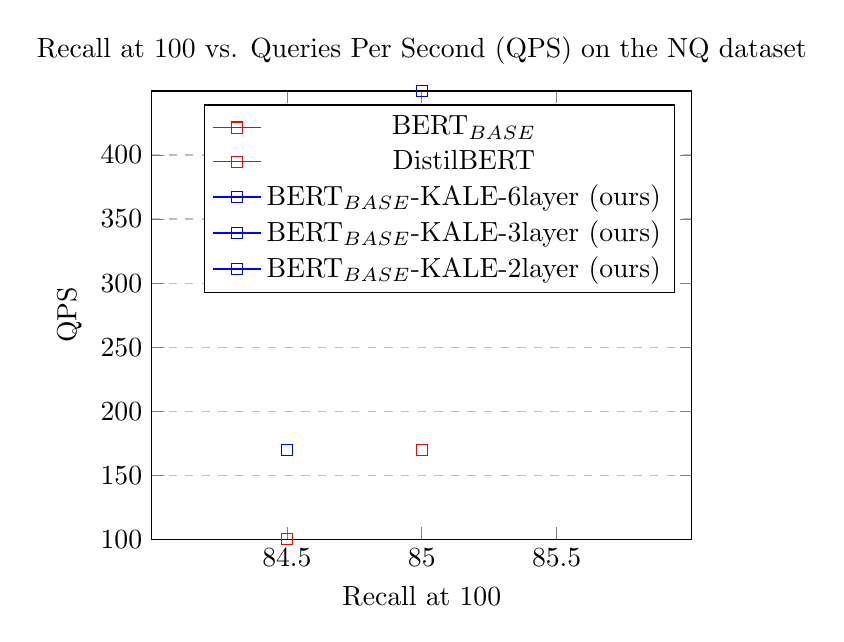
\begin{tikzpicture}
    \begin{axis}[
        title={Recall at 100 vs. Queries Per Second (QPS) on the NQ dataset},
        xlabel={Recall at 100},
        ylabel={QPS},
        xmin=84, xmax=86,
        ymin=100, ymax=450,
        xtick={84.5, 85, 85.5},
        ytick={100, 150, 200, 250, 300, 350, 400},
        legend pos=north east,
        ymajorgrids=true,
        grid style=dashed,
    ]
    
    % BERT_BASE
    \addplot[
        color=red,
        mark=square,
        ]
        coordinates {
            (84.5, 100)
        };
    \addlegendentry{BERT$_{\text{BASE}}$}
    
    % DistilBERT
    \addplot[
        color=red,
        mark=square,
        ]
        coordinates {
            (85, 170)
        };
    \addlegendentry{DistilBERT}
    
    % BERT_BASE-KALE-6layer (ours)
    \addplot[
        color=blue,
        mark=square,
        ]
        coordinates {
            (85.5, 300)
        };
    \addlegendentry{BERT$_{\text{BASE}}$-KALE-6layer (ours)}
    
    % BERT_BASE-KALE-3layer (ours)
    \addplot[
        color=blue,
        mark=square,
        ]
        coordinates {
            (84.5, 170)
        };
    \addlegendentry{BERT$_{\text{BASE}}$-KALE-3layer (ours)}
    
    % BERT_BASE-KALE-2layer (ours)
    \addplot[
        color=blue,
        mark=square,
        ]
        coordinates {
            (85, 450)
        };
    \addlegendentry{BERT$_{\text{BASE}}$-KALE-2layer (ours)}
    
    \end{axis}
\end{tikzpicture}

\end{document}